\section{\centering Normalization \& The Church-Rosser Theorem}
In this section we attempt to give the reader an overview of the properties behind this calculus. We analyze what makes the untyped \lcalc \ a suitable computation model, and provide enough evidence that it is missing some desirable properties that motivate the introduction of typing.

\subsubsection{\centering  The Church-Rosser Theorem}
To this end we specify some properties general to relations, specifically, those that help us reason about confluence and termination.

\begin{definition}
  Let $R \subseteq A \times A$ be a binary relation on a set $A$. The reflexive-transitive closure of $R$, denoted by $R^{*}$, is the smallest relation on $A$ such that:
  \[
  \begin{aligned}
    &\text{(Reflexivity)} && (x, x) \in R^{*} \\
    &\text{(Transitivity)} && (x, y) \in R^{*} \wedge (y, z) \in R^{*} \Rightarrow (x, z) \in R^{*} \\
    &\text{(Inclusion of $R$)} && (x, y) \in R \Rightarrow (x, y) \in R^{*}
  \end{aligned}
\]
where $x, y, z \in A$.
\end{definition}
\begin{note}
  $R^*$ contains all pairs that relate to each other in such a way that $x$ can be transformed into $y$ by applying $R$ zero or more times.
\end{note}
\begin{definition}  
Let $\to$ be a binary relation on a set $A$. The symbol $\to^{*}$ denotes reflexive-transitive closure of $\to$. We define the following properties:
\[
  \begin{aligned}
    &\text{(Church-Rosser)} && x \to^{*} y \wedge x \to^{*} z \Rightarrow \exists w \in A,\; y \to^{*} w \wedge z \to^{*} w \\
    &\text{(Quasi-Diamond)} && x \to y \wedge x \to z \Rightarrow \exists w \in A,\; y \to^* w \wedge z \to^* w \big. \\
    &\text{(Diamond)} && x \to y \wedge x \to z \Rightarrow \exists w \in A,\; y \to w \wedge z \to w
  \end{aligned}
\]
where $x, y, z, w \in A$.
\end{definition}
\begin{note}
  Both Church-Rosser and Quasi-Diamond are weaker than Diamond. Notice how Diamond $\Rightarrow$ Quasi-Diamond and Diamond $\Rightarrow$ Church-Rosser.
\end{note}

\begin{definition}
  The parallel $\beta$-reduction relation $M \Longrightarrow_\beta N$ is defined inductively by the following inference rules:
  \[
    \begin{array}{@{}l@{\quad}l@{}}
      \inferrule*[right=\textsc{Beta}]
      { N \Longrightarrow_\beta N' \\ Q \Longrightarrow_\beta Q' }
      { (\lambda x. N)\,Q \Longrightarrow_\beta N'[x:=Q'] }
      &
        \inferrule*[right=\textsc{Var}]
        { }
        { x \Longrightarrow_\beta x }\\[2ex]
      \inferrule*[right=\textsc{Abs}]
      { N \Longrightarrow_\beta N' }
      { \lambda x. N \Longrightarrow_\beta \lambda x. N' }
      &
        \inferrule*[right=\textsc{App}]
        { P \Longrightarrow_\beta P' \\ Q \Longrightarrow_\beta Q' }
      { P\,Q \Longrightarrow_\beta P'\,Q' }
    \end{array}
  \]
  Parallel $\beta$-reduction is assumed to be reflexive i.e. $ M \Longrightarrow_\beta M $
\end{definition}

\begin{note}
Notice how parallel $\beta$-reduction can simulate plain $\beta$-reduction. This fact will be used to prove properties for $\beta$-reduction.
\end{note}

\begin{definition} The complete development $M^*_\beta$ of a term $M$ is obtained by reducing all $\beta$-redexes in $M$ simultaneously:
\[
x^*_\beta = x, \quad
(\lambda x. N)^*_\beta = \lambda x. N^*_\beta, \quad
(PQ)^*_\beta = 
\begin{cases}
N^*_\beta[x := Q^*_\beta] & \text{if } P = \lambda x. N\\
P^*_\beta Q^*_\beta & \text{otherwise}
\end{cases}
\]
\end{definition}

\begin{lemma}
  \label{lemma:parallel-reduction}
  If $M \Longrightarrow_\beta M'$, then $M' \Longrightarrow_\beta M^*_\beta$.
  \begin{proof}[Proof Sketch]
    By induction on the derivation of $M \Longrightarrow_\beta M'$:
    \begin{itemize}
    \item $M = x$. Trivial: $M' = x = M^*_\beta$.
    \item $M = \lambda x.N$, $M' = \lambda x.N'$. By IH, $N' \Longrightarrow_\beta N^*_\beta$, so $\lambda x.N' \Longrightarrow_\beta \lambda x.N^*_\beta = M^*_\beta$.
    \item $M = PQ$, $M' = P'Q'$. By IH, $P' \Longrightarrow_\beta P^*_\beta$ and $Q' \Longrightarrow_\beta Q^*_\beta$.
      \begin{enumerate}
      \item If $P = \lambda x.N$, then $P' = \lambda x.N'$. By IH, $N' \Longrightarrow_\beta N^*_\beta$ and $Q' \Longrightarrow_\beta Q^*_\beta$. Apply the redex rule: $P'Q' = (\lambda x.N')Q' \Longrightarrow_\beta N^*_\beta[Q^*_\beta/x] = M^*_\beta$.
      \item If $P$ is not a $\lambda$-abstraction, then $P'Q' \Longrightarrow_\beta P^*_\beta Q^*_\beta = M^*_\beta$.
      \end{enumerate}
    \item $M = (\lambda x.N)Q$, $M' = N'[Q'/x]$. By IH, $N' \Longrightarrow_\beta N^*_\beta$ and $Q' \Longrightarrow_\beta Q^*_\beta$. Substitution preserves parallel reduction: $N'[Q'/x] \Longrightarrow_\beta N^*_\beta[Q^*_\beta/x] = M^*_\beta$.
    \end{itemize}
  \end{proof}
\end{lemma}
\begin{remark}
This lemma formalizes the fact that a single parallel $\beta$-reduction step does not miss any $\beta$-redexes: after reducing in parallel to $M'$, one can still reach the complete development $M^{\beta\ast}$ of the original term by further parallel $\beta$-reductions. In other words, parallel $\beta$-reduction is complete with respect to the simultaneous contraction of all redexes---no matter which parallel step you take, the term remains on a path toward the fully developed form.
\end{remark}

\begin{theorem} The Church-Rosser Theorem states that if $M \curly^* N_1$ and $M \curly^* N_2$, then there exists $P$ such that
\[
N_1 \curly^* N_3 \quad \text{and} \quad N_2 \curly^* N_3.
\]
Graphically:
  \begin{center}
    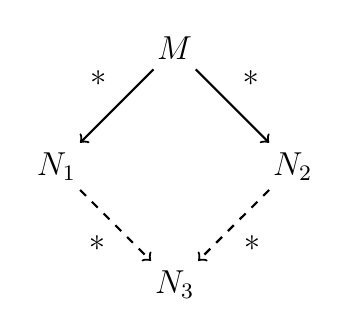
\begin{tikzpicture}[node distance=2.0cm, every node/.style={font=\large}]
      \node (t) at (0,0) {$M$};
      \node (t1) at (-1.5,-1.5) {$N_1$};
      \node (t2) at (1.5,-1.5) {$N_2$};
      \node (t3) at (0,-3) {$N_3$};
      \draw[->, thick] (t) -- (t1) node[midway, above left] {*}; %{$\curly^*$};
      \draw[->, thick] (t) -- (t2) node[midway, above right] {*}; %{$\curly^*$};
      \draw[->, dashed, thick] (t1) -- (t3) node[midway, below left] {*}; %{$\curly^*$};
      \draw[->, dashed, thick] (t2) -- (t3) node[midway, below right] {*}; %{$\curly^*$};
    \end{tikzpicture}
  \end{center}
\end{theorem}

\begin{proof}
Any $\beta$-reduction can be simulated by parallel reduction. Suppose $M \Longrightarrow_\beta N_1$ and $M \Longrightarrow_\beta N_2$. By lemma \ref{lemma:parallel-reduction},
\[
N_1 \Longrightarrow_\beta M^*_\beta \quad \text{and} \quad N_2 \Longrightarrow_\beta M^*_\beta.
\]
Parallel reduction implies ordinary multi-step $\beta$-reduction: $N_1 \curly^* M^*_\beta$ and $N_2 \curly^* M^*_\beta$. Hence $M^*_\beta$ is a common reduct.
\end{proof}

\begin{remark}
  The untyped \lcalc \ does not obey the Diamond property. The proof of this fact is given later on when we present fixed points and recursion \ref{}.
\end{remark}

\begin{corollary} Normalization: If a $\lambda$-term $M$ reduces to two normal forms $N_1$ and $N_2$, then they are unique up to alpha-equivalece:
\[
M \curly^* N_1 \ \ \text{and} \ \ M \curly^* N_2 \ \ \text{and $N_1$, $N_2$ are normal} \ \ \Rightarrow \ \ N_1 =_\alpha N_2
\]
\end{corollary}

\begin{proof}[Proof]
By the Church-Rosser theorem, there exists a term \( P \) such that
\(
N_1 \curly^{*} P \quad \text{and} \quad N_2 \curly^{*} P.
\)
Since \( N_1 \) and \( N_2 \) are normal forms, they cannot be reduced further.  
Thus, the only possible \( P \) is \( N_1 =_\alpha N_2 \).
\end{proof}

Looking at the big picture, we find this normalization property to be a non-trivial result that helps us verify that the \lcalc \ is a deterministic model of computation. Meaning that if we take a program and run it, it will always give the same output for a given input. Of course, when we say a program, we mean a \lterm, and when we say run, we mean $\beta$-reduce. Perhaps the following section enables the reader to better grasp why we informally speak of lambda terms as programs.


\begin{remark}
  \cite{nagele2016mechanized} is a mechanized proof of the Church-Rosser Theorem using the $Z$-property written in Nominal Isabelle.
\end{remark}


\subsubsection{\centering Normalization}

Normalization properties essentially summarize the termination properties of terms in the context of $\beta$-reduction.

\begin{definition} Consider a lambda term \(M\) and all possible \(\beta\)-reduction sequences
\[
  M \equiv M_0 \curly M_1 \curly \cdots \curly M_n
\]
\[
  M \equiv N_0 \curly N_1 \curly \cdots \curly
\]
\[
  \cdots
\]
We classify \(M\) as follows:
\begin{itemize}
    \item \(M\) is strongly normalizing if every such reduction sequence terminates in a normal form. Equivalently, there is no infinite reduction sequence.
    \[
    M \equiv M_0 \curly M_1 \curly M_2 \curly \cdots
    \]
    \item \(M\) is weakly normalizing if there exists at least one finite reduction sequence     that terminates in a normal form.
    \[
    M \equiv M_0 \curly \cdots \curly M_n
    \]
    \item \(M\) is non-normalizing if no reduction sequence starting from \(M\) ever reaches a normal form. In this case, every reduction path is either infinite or loops without producing a normal form.
\end{itemize}
\end{definition}
\begin{proposition}
  A term may be either, weakly normalizing, strongly normalizing or non-normalizing.
\end{proposition}
\begin{proof} Examples are:
\begin{enumerate}
\item \(\lambda x. x\) is strongly normalizing since it is already in normal form.
\item \(\Omega = (\lambda x. x x)(\lambda x. x x)\) reduces to itself forever, hence non-normalizing.
\item \((\lambda x. y)\, \Omega \curly y\), so it has a normal form \(y\), but reducing \(\Omega\) loops, so it is weakly normalizing.
\end{enumerate}
\end{proof}
\begin{remark}
  Checking whether a term is terminating is undecidable in general, since it is an instance of the halting problem.
\end{remark}



